%%%%%%%%%%%%%%%%%%%%%%%%%%%%%%%%%%%%%%%%%%%%%%%%%%%%%%%%%%%%%%%%%%%%%%%%%%%%%%%%
%2345678901234567890123456789012345678901234567890123456789012345678901234567890
%        1         2         3         4         5         6         7         8

\documentclass[letterpaper, 10 pt, conference]{ieeeconf}  % Comment this line out if you need a4paper

%\documentclass[a4paper, 10pt, conference]{ieeeconf}      % Use this line for a4 paper

\IEEEoverridecommandlockouts                              % This command is only needed if
                                                          % you want to use the \thanks command

\overrideIEEEmargins                                      % Needed to meet printer requirements.

% See the \addtolength command later in the file to balance the column lengths
% on the last page of the document

\usepackage{graphicx} % needed to include png files
\usepackage{multirow} % for the table

% The following packages can be found on http:\\www.ctan.org
\usepackage{graphics} % for pdf, bitmapped graphics files
% \usepackage{epsfig} % for postscript graphics files
% \usepackage{mathptmx} % assumes new font selection scheme installed
% \usepackage{times} % assumes new font selection scheme installed
% \usepackage{amsmath} % assumes amsmath package installed
% \usepackage{amssymb}  % assumes amsmath package installed

\title{\LARGE \bf
Mesh Adition Based on the Depth Image (MABDI)
}


\author{Lucas Chavez$^{1}$ and Ron Lumia$^{2}$% <-this % stops a space
\thanks{*This work was not supported by any organization}% <-this % stops a space
\thanks{$^{1}$Lucas is with Mechanical Engineering Department and Electrical \& Computer Engineering Department, University of New Mexico,
	Albuquerque, NM, USA
        {\tt\small \{lucasc,lumia\}@unm.edu}}%%
}


\begin{document}



\maketitle
\thispagestyle{empty}
\pagestyle{empty}


%%%%%%%%%%%%%%%%%%%%%%%%%%%%%%%%%%%%%%%%%%%%%%%%%%%%%%%%%%%%%%%%%%%%%%%%%%%%%%%%
\begin{abstract}

% introspection
% classification
% using mesh methods

Many robotic applications, especially those whose goal is to aid or assist
through human robot interaction, utilize a rich map of the world for reasoning
tasks such as collosion detection, path planning, or object recognition. Such
map, and the method used to produce it, must take into consideration real-world
constraints. Most mesh-based mapping algorithms resemple a ``black box'' and do
no provide a mechanism to close the loop and make decisions about the
incoming information. MABDI leverages the global mesh by finding the difference
between what we expect to see and what we are actually seeing, and using this to
classify the incoming measurements as novel or not. This allows the surface
reconstruction method to be run only on data that hasn't yet been represented in
the global mesh. Resulting in an algorithm that becomes computationally
inexpensive once the environment is known, but can also react to new objects.


\end{abstract}


\section{Introduction} \label{sec:introduction}

Many robotic applications, especially those that involve human robot interaction, often require a rich representation of the environment in order to perform such behavior as path planning and obstacle avoidance. In general, a rich representation, or map, is useful for providing situational awareness to an autonomous agent. A map is also important for applications such as teleoperation \cite{Kadous2006}.

The methodology to build this
representation is a continuously evolving subject in the field of robotics.
The origins of the research into this problem dates back roughly 25 years \cite{Lorensen1987}.
Since then the methods and the representations themselves have continued to
evolve at an impressive rate. The main catalyst behind this growth is the
advancement of sensing technologies over the same time period. In general,
sensors have continued to generate measurements at higher rates, higher
resolution, and lower cost over the years. This has provided an amazing
opportunity to build richer and more useful representations of the
environment.

In robotics map building in an unknown environment is referred to as
the Simultaneous Localization and Mapping (SLAM) problem \cite{Thrun2002}. This label
describes the fact that a methodology which solves the SLAM problem must
simultaneously locate the robot in the environment as well as map the
environment. The focus of this work is the mapping aspect of the SLAM problem. Fig. \ref{fig:goal} gives a visualization of the goal.

\begin{figure}[h]%[thpb]
\centering
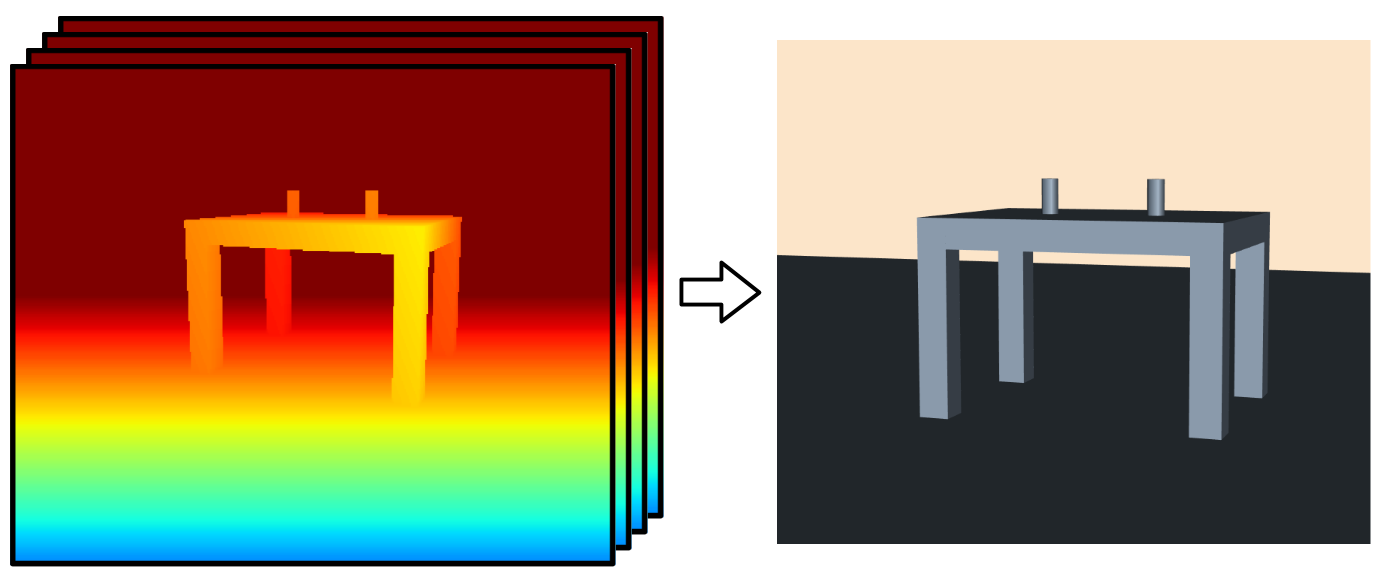
\includegraphics[width=.5\textwidth]{figures/diagram_goal.png}
\caption{Goal is to create a map from depth images}
\label{fig:goal}
\end{figure}


There are different types of data structures that can define a map. All of which have intrinsic characteristics that impact the algorithms that generate them and create constraints that must be considered for real-world applications. In addition, we are concerned with rich representation types, in contrast to sparse representation types \cite{Dissanayake2001}, because rich types have the most use in applications such as human robot interaction.

\begin{table}[h]
\begin{footnotesize}
\begin{center}
\begin{tabular}{|l|c|c|c|c|c|}
\hline
\multirow{2}{*}{} & Supported & Computationally & Low Memory \\
 & & Inexpensive & Requirement \\\hline
Point Clouds		& x & x & - \\
Surfels             	& - & x & x \\
Implicit Functions 	& x & - & - \\
Mesh	 	& x & x & x \\
\hline
\end{tabular}
\end{center}
\end{footnotesize}
\caption{Comparison of constraints for different map types}
\label{tab:rep}
\end{table}

When considering what type of map is best for real-world applications, we must consider the constraints imposed by each type:

\begin{itemize}
\item Supported - Is there software, tools, research, algorithms, etc. for this type of map?
\item Computationally Inexpensive - Can the algorithms be run on cost effective hardware?
\item Low Memory Requirement - Can the algorithms be run on hardware with standard process memory?
\end{itemize}

Table \ref{tab:rep} compares the constraints of common map types. We can see, in
general a mesh type map satisfies real-world constraints. It has been used
extensively by the gaming and graphics communities, and so benefits from an
incredible amount of continued research and advances in hardware such as GPUs.

Currently, one of the issues with mesh mapping techniques is they are generally
``black box'' methods. Meaning the data comes in from the sensor, those
measurements are turned into a mesh, and then that mesh is appended to a global
mesh. Fig. \ref{fig:pipeline} visualizes this common pipeline in black. The goal
of this work is to design an algorithm to close the loop (as visualized in red)
and allow the system to make decisions about the incoming data based on what it
already knows.

\begin{figure}[h]%[thpb]
\centering
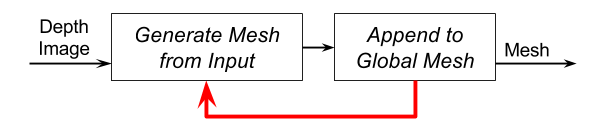
\includegraphics[width=.5\textwidth]{figures/diagram_general_pipeline.png}
\caption{Common ``black box'' pipeline in black. The contribution of MABDI in red.}
\label{fig:pipeline}
\end{figure}

% set up what environmental mapping is, what a mesh is
% design goals of the system

\section{Related Works}	\label{sec:related_works}

Works related to MABDI are generally based on RGB-D sensors. This type of sensor has
become very popular since the release of the Kinect from Microsoft TODO ref, which
was the first mass produced RGB-D sensor of its kind. RGB-D sensors are
inexpensive and produce noisy 640x480 depth images at 30fps. The RGB-D
sensor has excited the robotics community because this has been the first
time that depth data has been so readily accessible from such an
inexpensive sensor. Therefore, these methodologies must be able to quickly
deal with very high rates of information.

One very impressive work came
from Henry et al. in 2012 \cite{Henry2012}. In this work they designed a
system which used a RGB-D sensor to build a map made of surfels. In order to
generate and maintain the surfel map they used the work of Weise et al.
\cite{Weise2009}. Surfels are circular disks which have a particular
position and orientation and also a radial size based on confidence. The
map consists of a large number of surfels. The surfel map can be updated
given the new registered depth images from the sensor. Decisions are made
of how to handle each measurement in the depth image based on the
difference between an expectation generated using the current map and the
actual readings from the sensor. Rendering a surfel map requires special
methods \cite{Pfister2000} and is difficult to use in applications such as
obstacle avoidance.

One of the next major advances was published by Whelan
et al. in 2012 \cite{Whelan2012} and more recently in 2013
\cite{Whelan12tr}. The system they developed was named Kintinuous and was
able to produce a high quality mesh representation of the environment.
Their system was a hybrid system and utilized the KinectFusion method
\cite{Newcombe2011a} of Newcombe et al. to create a volumetric
representation of the portion of the environment in front of the sensor. As
the sensor moves, portions of the environment that leave the volume in
front of the sensor are ray cast and turned into a mesh. They obtain very
impressive results but also mention a limitation of their system for future
work. The limitation is that the mesh can not be updated once created,
which is an issue when revisiting parts of the environment. One of the most
impressive current works which has an adaptable mesh came from Cashier et
al. in 2012 \cite{Cahier2012}. In this work, they were able to generate and
update a mesh with new measurements from a ToF sensor. They used the
difference between the existing model and the actual measurements to decide
whether to adapt the mesh or add new elements. The mesh topology was not
adaptive to the environment and their experiments only showed results of mapping a
single flat wall with no robot movement. The system needs to be tested for
object addition and removal.

Research and development of new mapping algorithms are trending towards
leveraging the information in the global map to make decisions about the
incoming data. One can see parallels with how we as humans see the world. MABDI
proposes do this in a computationally feasible way by using simply using
differencing and thresholding imaging methods.

% show many mesh based algorithms are black box
% systems capable of introspection such as kinectfusion rely on volumetric
% representation and are computationally and memory expensive

\section{Approach}	\label{sec:related_works}

The algorithmic structure of MABDI can be seen in Fig. \ref{fig:system}. The diagram is very similar to Fig. \ref{fig:pipeline} with the exception of the Classification component, shown in blue. This Classification component is MABDI's contribution to the state-of-art in mesh based mapping algorithms, and is what gives MABDI the ability to make decisions about the incoming data.

The Classification component consists of two elements:
\begin{enumerate}
    \item \textit{Generate Expected Depth Image $E$} - Here we take the global
    mesh $M$, render it using computer graphics, and use the depth buffer of the
    render window to create a depth image $E$ of what we expect to see from our
    sensor. This method requires the current pose $P$ of the actual sensor
    (simulated for our experiments).
    \item \textit{Classify Depth Image $D$} - Here we classify the actual depth
    image $D$ (simulated for our experiments) by first taking the absolute
    difference between $E$ and $D$ and thresholding. If the differences are
    small, those points are thrown away and if the differences are large, those
    points are kept as $D_n$. The idea behind this is, if the difference is
    large, the measurements are coming from a part of the environment that has
    not been seen before i.e. novel. The implication of is assumption, is that
    this version of MABDI can not handle object removal. It is worth noting,
    that MABDI can be extended to handle object removal by using the sign of the
    difference between $E$ and $D$ instead of the absolute value.
\end{enumerate}

\begin{figure}[h]%[thpb]
\centering
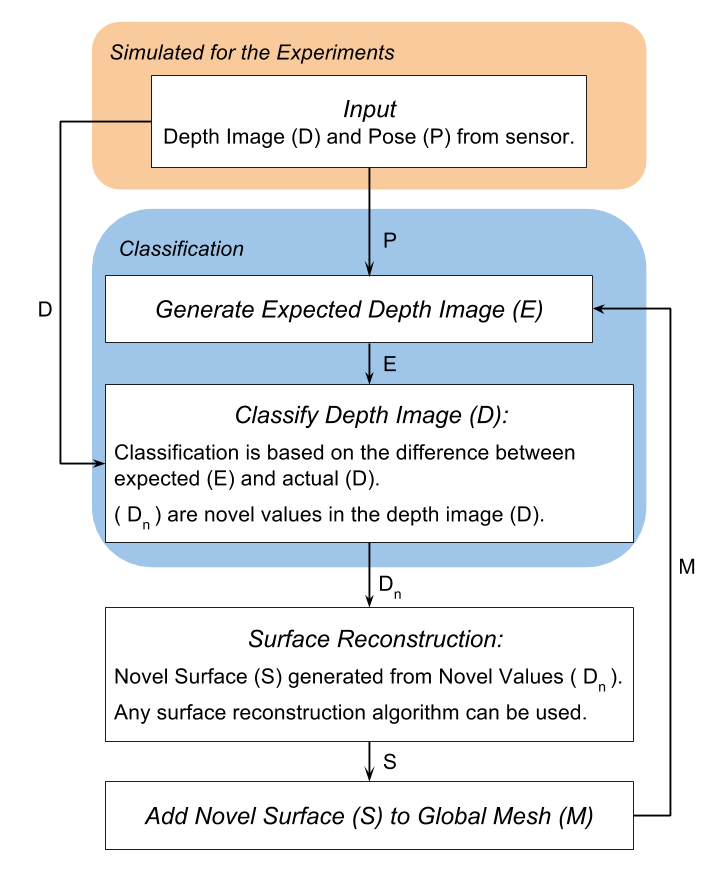
\includegraphics[width=.5\textwidth]{figures/diagram_system.png}
\caption{MABDI system diagram}
\label{fig:system}
\end{figure}



\begin{figure}[h]%[thpb]
\centering
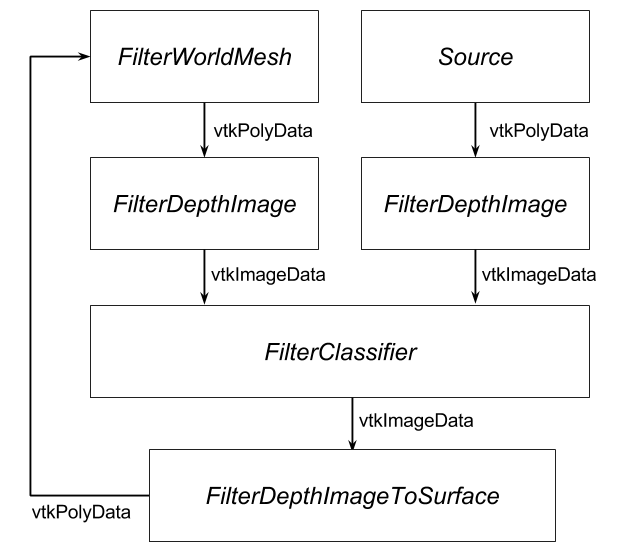
\includegraphics[width=.5\textwidth]{figures/diagram_software.png}
\caption{MABDI software diagram}
\label{fig:software}
\end{figure}

% How Mabdi works, describe the algorithm
% How Mabdi is implemented

\section{Experimental Setup}	\label{sec:related_works}

\begin{figure}[h]%[thpb]
\centering
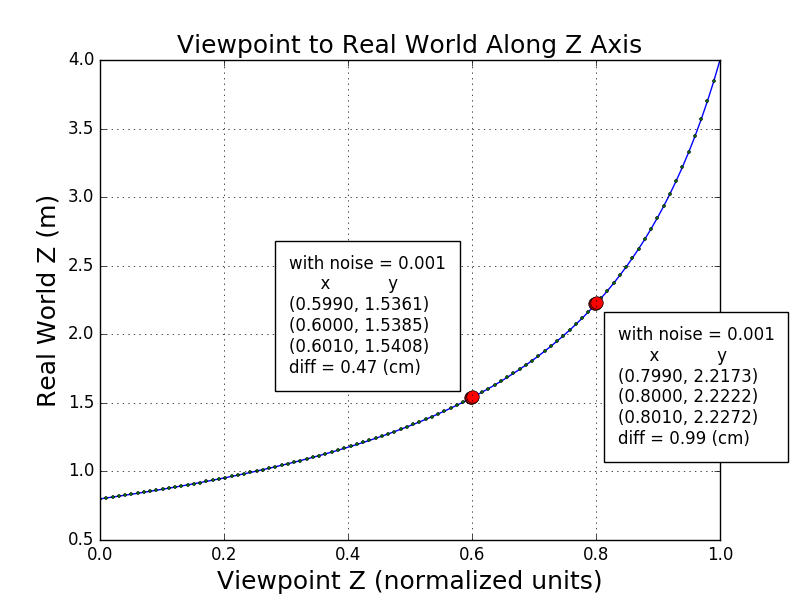
\includegraphics[width=.5\textwidth]{figures/plot_depth.png}
\caption{Viewpoint coordinates to real world coordinates analysis. Viewpoint coordinates are obtained when a mesh is rendered into a render window, and can be transformed to real-world coordinates using the transformation matrix of the camera. Noise is added in simulation to the viewpoint coordinates. This graph shows the effect of that noise in real-world coordinates.}
\label{fig:pipeline}
\end{figure}

% describe the simulation environment
% maybe determine speed of walker
% discuss noise

% \section{Results} \label{sec:results} 

With the captured data, it was possible to fill 72.9\% of the original
neighborhoods with, at least, a threshold of 500 points. The distribution of
number of points across the $X$ space is illustrated by Figure
\ref{fig:numberOfPointsPerBin}.

We performed a quantile-quantile regression with the data shown in the
histogram from Figure \ref{fig:distancesToPlane} with a gaussian distribution,
and obtained a coefficient of determination of 0.805, which validates the
hypothesis that the error $e_i$ can be approximated by a Gaussian random
variable with zero mean.  Figure \ref{fig:sampleMeanFigure} shows the average
of the error calculated from the samples at each neighborhood $N_j$. Since most
of its values are dispersed close to zero, we can say that the approximation of
a zero-centered distribution for each neighborhood does not compromise our
model, whilst making it simpler for real applications.

Next we will show the results of our model generation. In Figure \ref{fig:stdImageZeroMean} we can see
the variance $\sigma_j$ in each neighborhood $N_j$ and observe that $\sigma_j$
increases with distance, which is a trend we expected. One important
observation is that, according to our model, the angle $\alpha$ does not play a
major role in determining the variation $\sigma_j$.  In Figure \ref{fig:scatterWithZeroMean} we can see a
scatter plot showing our generated polynomial surface $\sigma(\alpha,d)$;
$\sigma_j$ obtained from our data set; and $\sigma_j$ obtained from our
validation set. The surface represents the best fit polynomial surface through
the original estimations. The green dots represent the original estimations;
the red ones were acquired from the XtionPRO, while the black points were
computed from a different Kinect sensor.

We asses the ability of our model to describe our data by the coefficient of
determination. This allows us to determine the percentage of points whose
variation are described by $\sigma(\alpha,d)$. In Table \ref{tab:CD_coefs} we
can see the value of this coefficient for our large data set and also our
validation set. Our results show that our model could be used for other
Kinect device with a reasonable confidence, but that a new model would be needed
for the Xtion, should the application require a high accuracy model. 

%{\setlength\abovedisplayskip{-4pt} \setlength\belowdisplayskip{-6pt} % needed to make spacing more compact
\begin{table}[h!]
\caption{Coefficient of determination.}
\begin{center}
\begin{tabular}{|c|c|c|}
\hline
Original Kinect & Another Kinect & ASUS XtionPRO \\ \hline
$90.0\%\ $ & $74.7\%\ $ & $50.7\%\ $ \\ \hline
\end{tabular}
\end{center}
\label{tab:CD_coefs}
\end{table}
%}

The resulting measurement noise model from our analysis is given by (\ref{eq:model}) and the list of coefficients are in Table \ref{tab:Poly_coefs}.

{\setlength\abovedisplayskip{-4pt} \setlength\belowdisplayskip{-6pt} % needed to make spacing more compact
\begin{multline}
\sigma(d,\alpha) = A +  B \alpha  + Cd + D\alpha^2  + E\alpha d \\ +  Fd^2  + G\alpha^3   +H \alpha^2 d   +I\alpha d^2    +Jd^3
\label{eq:model}
\end{multline}
}

%{\setlength\abovedisplayskip{-4pt} \setlength\belowdisplayskip{-6pt} % needed to make spacing more compact
\begin{table}[h]
\caption{Polynomial coefficients for the surface $\sigma(d,\alpha)$.}
\begin{center}
\begin{tabular}{|c|c|c|c|}
\hline
$A$ & $0.0125$ & $F$ & $0.0037$ \\ \hline
$B$ & $-6.0904\times 10^{-4}$ & $G$ & $3.4986 \times 10^{-8}$ \\ \hline
$C$ & $-0.0061$ & $H$ & $-3.9492 \times 10^{-6}$ \\ \hline
$D$ & $8.0999\times 10^{-6}$ & $I$ & $-2.7408 \times 10 ^{-6} $ \\ \hline
$E$ & $1.5757 \times 10^{-4}$ & $J$ & $-1.1158 \times 10^{-4}$ \\
\hline
\end{tabular}
\end{center}
\label{tab:Poly_coefs}
\end{table}
%}

\setlength\figureheight{.25\textwidth} 
\setlength\figurewidth{.4\textwidth}
\begin{figure}[h]
\centering 
\beginpgfgraphicnamed{tikzExt/distancesToPlane} 
\input{tikzFigs/distancesToPlane.tikz} 
\endpgfgraphicnamed 
\caption{ 
Histogram of the error $e_i$ for all the points $p_i$ in our data set. This shows that a normal distribution is a good approximation to our data.
} 
\label{fig:distancesToPlane}
\end{figure} 

\setlength\figureheight{0.31603\textwidth} 
\setlength\figurewidth{ 0.238  \textwidth}
\begin{figure}[p]
\centering 
\beginpgfgraphicnamed{tikzExt/numberOfPointsPerBin} 
\input{tikzFigs/numberOfPointsPerBin.tikz} 
\endpgfgraphicnamed 
\caption{ 
Number of points in each neighborhood $N_j$. In this image, each neighborhood is represented by a pixel centered at the neighborhood centroid. 
} 
\label{fig:numberOfPointsPerBin}
\end{figure} 

\setlength\figureheight{0.31603\textwidth} 
\setlength\figurewidth{ 0.238  \textwidth}
\begin{figure}[p]
\centering 
\beginpgfgraphicnamed{tikzExt/sampleMeanFigure} 
\input{tikzFigs/sampleMeanFigure.tikz} 
\endpgfgraphicnamed 
\caption{ 
Mean value of $e_i$ in each neighborhood $N_j$ which we define as $\overline{e_k}$. In our analysis we set this value equal to zero. This graph gives some experimental justification for this assumption.   
} 
\label{fig:sampleMeanFigure}
\end{figure} 

\setlength\figureheight{0.31603\textwidth} 
\setlength\figurewidth{ 0.238  \textwidth}
\begin{figure}[p]
\centering 
\beginpgfgraphicnamed{tikzExt/stdImageZeroMean} 
\input{tikzFigs/stdImageZeroMean.tikz} 
\endpgfgraphicnamed 
\caption{ 
Values for standard deviation $\sigma_j$ at each neighborhood. We can see the variance increases with larger values distance $d$ while being weakly influenced by the incident angle $\alpha$.
} 
\label{fig:stdImageZeroMean}
\end{figure} 

%\setlength\figureheight{.28\textwidth} 
%\setlength\figurewidth{.28\textwidth}
%\begin{figure}[h]
%\centering 
%%\beginpgfgraphicnamed{tikzExt/scatterWithZeroMean} 
%\input{tikzFigs/stdImageZeroMean.tikz} 
%%\endpgfgraphicnamed 
%\caption{ 
%Standard deviation of $e_i$ in each neighborhood $N_j$, using $\mu=0$
%} 
%\label{fig:stdImageZeroMean}
%\end{figure} 

% had to edit tikz file
%  - comment every other line of surface out
%  - use "hot" instead of "jet"
%  - specify "mark size=.3pt" in addplot3
\pgfplotsset{xlabel shift = -1ex}
\pgfplotsset{ylabel shift = -1ex}
\setlength\figureheight{.35\textwidth} 
\setlength\figurewidth{.32\textwidth}
\begin{figure}[p]
\centering 
\beginpgfgraphicnamed{tikzExt/scatterWithZeroMean} 
\input{tikzFigs/scatterWithZeroMean.tikz} 
\endpgfgraphicnamed 
\caption{ 
Our noise model for the Kinect. The dots represent the local estimation of $\sigma$ for a particular neighborhood $N_j$. 
} 
\label{fig:scatterWithZeroMean}
\end{figure} 



% Results of the runs
% Definitely talk about how adding a bunny worked well

% \section{Conclusion} \label{sec:conclusion} 

% this work presents 
% by ...

% needs:
% created a measurement noise model 
% cheap method to estimate "ground truth"
% generated model which would will be more accurate then ad hoc models
% our model should work for other Kinect sensors reasonably well
% maybe need to regenerate if have an ASUS
% we provide our methodology so that one can do that
% future work - apply to KinectFusion

This work has presented a novel methodology for generating a measurement noise
model for Kinect-style sensors.  Classical work in sensor modeling has defined
the uncertainty to be constant for all measurements. For many depth sensors,
especially those like Kinect, this constant assumption simply isn't true. In
recent work ad hoc models have been created to be more realistic. Our method
generates sensor models from a thorough stochastic analysis of a large data
set. We give our generated model and compare the results with a validation set.
Our method is better than an ad hoc guess, however a model may need to be
generated for a specific sensor depending on the needs of the algorithm it will
be used for. We have made it easy to generate a model for your own sensor by
making the code freely available. In future work we intend to improve our model
by taking into account the error induced by lens distortion. Additionally, we
would like to evaluate our model with existing SLAM algorithms.

% discuss difficulty with noise
% how to expand to deal with object deletion

%%%%%%%%%%%%%%%%%%%%%%%%%%%%%%%%%%%%%%%%%%%%%%%%%%%%%%%%%%%%%%%%%%%%%%%%%%%%%%%%

\bibliographystyle{IEEEtran}
\bibliography{bibliography}

\end{document}
